\documentclass[10pt,oneside,a4paper,final,english]{memoir}

\usepackage{palatino}
\usepackage{microtype}
\usepackage{lscape}
\usepackage{multicol}
%\usepackage{epic,eepic}
\usepackage{latexsym}
\usepackage{verbatim}
\usepackage{listings}
\usepackage{ulem}
\usepackage{hyperref}

\let\footruleskip\undefined
\usepackage{fancyhdr}
\usepackage[final]{fixme}

\let\fref\undefined
\usepackage[plain]{fancyref}

%% FOR LOOP
\usepackage{ifthen,calc}
\newcounter{myforloopcounter}
\newcommand{\forloop}[5][1]% 
{\setcounter{#2}{#3}% 
\ifthenelse{#4}% 
{#5%
  \addtocounter{#2}{#1}% 
  \forloop[#1]{#2}{\value{#2}}{#4}{#5}% 
}%
% Else 
{}%
}% 


%% USAGE
%\forloop[step]{counter}{initial_value}{conditional}{code_block} 
\usepackage[english]{babel}
\usepackage[utf8]{inputenc}

%\selectlanguage{danish}

\lstset{language=Python,basicstyle=\small,
  columns=fullflexible}


\usepackage[pdftex]{graphicx}

\DeclareGraphicsExtensions{.jpg .png .pdf}


\usepackage{amsmath}
\usepackage{latexsym}
\usepackage{amssymb}


\usepackage[osf,sc]{mathpazo}
\usepackage{microtype}
%\usepackage{fourier}
\linespread{1.05}

%\usepackage[charter]{mathdesign}
%\usepackage{lmodern}

%\usepackage{algorithmic}
%\usepackage{algorithm}

\usepackage{amsthm}


\theoremstyle{plain}  \newtheorem{definition}{Definition}
\theoremstyle{remark} \newtheorem{lemma}{Lemma}
\theoremstyle{plain}  \newtheorem{theorem}{Theorem}
\theoremstyle{remark}  \newtheorem{example}{Example}


\newcommand{\p}{\ensuremath{^\prime}}
\DeclareGraphicsExtensions{.jpg, .eps, .png}
%%% Local Variables:
%%% mode: plain-tex
%%% TeX-master: "../master"
%%% End:

\usepackage{algorithmic}
\usepackage{algorithm}
\usepackage[sectionbib,square]{natbib}
%\bibpunct{(}{)}{,}{a}{}{}
\setcitestyle{alpha}
%\setcitestyle{numbers,aysep={},yysep={;}}

\usepackage{datetime}

%\chapterstyle{thatcher}

%\setcounter{chapter}{1}
%\setcounter{secnumdepth}{1}
\setcounter{tocdepth}{2}




%\pagestyle{fancy}
\begin{document}
  \fontencoding{T1}
%  \fontseries{m}
%  \fontshape{n}
%  \fontsize{12}{15}
%  \selectfont


%%%%%%%%%%%%%%%%%%%%%%%%%%%%%%%%%%%%%%%%%%%%%%%%%%%%%%%%
%                    Forside
%%%%%%%%%%%%%%%%%%%%%%%%%%%%%%%%%%%%%%%%%%%%%%%%%%%%%%%%
\makeatletter % open mode for reading @ signed variables
\def\maketitle{%
 \null
 \thispagestyle{empty}%
 \vfill
 \begin{center}\leavevmode
   \normalfont
   \LARGE{\raggedleft \@title\par}%
   \hrulefill\par
   \large{\raggedleft \subtitle\par}%
   \vskip 2cm
   {\today\par}%
 \end{center}%
 \vfill
 \begin{flushleft}
   {\large \@author } \\
   {\footnotesize \suplementInfo }
 \end{flushleft}
 \clearpage % Terminates the page here. Everything else vil be placed
            % on next page.
}
\makeatother % closing mode for reading @ signed variables
%%%%%%%%%%%%%%%%%%%%%%%%%%%%%%%%%%%%%%%%%%%%%%%%%%%%%%%%
%               Data til forside
%%%%%%%%%%%%%%%%%%%%%%%%%%%%%%%%%%%%%%%%%%%%%%%%%%%%%%%%
\title{Final Hand In $\cdot$ Week VIII}

\def\subtitle{CCO $\cdot$ Constraint Continuous Optimization}

\author{Johan Sejr Brinch Nielsen} \def\suplementInfo{

\kern 5pt \hrule width 11pc \kern 5pt

\begin{tabular}{ll}
Email: & zerrez@diku.dk  \\
Cpr.:  & 260886-2547
\end{tabular}

% putter 5pt spacing oven over og neden under stregen
\kern 5pt \hrule width 11pc \kern 5pt

Dept. of Computer Science,  \\
University of Copenhagen

}


\maketitle
\newpage

\frontmatter
\tableofcontents
\newpage

\section{Introduction}
This weeks assignment is to perform a physics simulation of balls
falling and bouncing inside a box.


\section{Linear Complimentary Problems}
A linear complimentary problem (LCP) is a specific category of
optimization problems, which take the form:\\

\begin{center}\begin{tabular}{rl}
$A\lambda + b$ & $\geq 0$ \\
$\lambda$ & $\geq 0$\\
$\lambda^T (A\lambda + b)$ & $= 0$
\end{tabular}\end{center}

Where $A$ is a given matrix, $b$ is a given vector and $\lambda$ is
the solution vector that is to be found.


\section{Splitting Method}
\label{splitting}
The Splitting method solves a LCP by first splitting the matrix $A$ in
two. Hereafter, it defines a series of sub-problems which also belongs
to the LCP class. However, hopefully these are easy to solve.

The first step is to split $A$ into to new matrices $M$ and $N$ such
that:
\[ A = M - N \]

The sub-problem is now defined as:
\begin{center}\begin{tabular}{rl}
$M\lambda^{k+1} + c^k$ & $\geq 0$ \\
$\lambda^{k+1}$ & $\geq 0$\\
$(\lambda^{k+1})^T (M\lambda^{k+1} + c^k)$ & $= 0$
\end{tabular}\end{center}

Where $c^k = b - N\lambda^k$. Letting $M\lambda^{k+1}$ be $M\lambda^k$
makes the left-hand side of the first inequality become:
\[ M \lambda^k + c^k = M\lambda^k + b - N\lambda^k \]
\[ = A\lambda^k + b\]

And the sub-problem is back to the original LCP. Hence, the only
difference lies in using $\lambda^{k+1}$ together with $M$ and
$\lambda^k$ together with $N$. Since $\lambda^k$ is the approximation
of $\lambda^\star$ at iteration $k$, and $\lambda^{k+1}$ that at
iteration $k+1$, this is a fixed point computation yielding a solution
to the original LPC.

Not surprisingly, this fixed point iteration can be solved
iteratively. A bit more surprising is, that we need to apply the
minimum map reformulation. This reformulation yields the following
minimization problem:
\[ \min_\lambda (\lambda^{k+1}, M\lambda^{k+1} + c^k) = 0 \]
This formulation ensures the inequality constraints are fulfilled,
since neither can be negative (the smallest of the two must be
$0$). This is equivalent to the equality constraint, that ensures the
product of the two is $0$. Hence, the new formulation is the same
as the sub-problem.

We can now work on the new formulation:
\begin{center}\begin{tabular}{rlll}
    $ \min $ & $(\lambda^{k+1}, M\lambda^{k+1} + c^k)$&
    $ = 0 $ & $\Rightarrow $ \\

    $ \min $ & $(0, M\lambda^{k+1} + c^k - \lambda^{k+1}) $&
    $= -\lambda^{k+1} $ & $\Rightarrow $ \\

    $ \max $ & $(0, - M\lambda^{k+1} - c^k + \lambda^{k+1}) $&
    $= \lambda^{k+1} $ &
\end{tabular}\end{center}

The result is still a fixed point problem (it contains $\lambda^{k+1}$
on both sides). However, there is one more trick up the sleeve: case
analysis. I perform a case analysis on the sign of $S =
-M\lambda^{k+1} - c^k + \lambda^{k+1}$:

\paragraph{Case 1: } $S = -M\lambda^{k+1}-c^k+\lambda^{k+1} < 0$\\
If this is the case $\lambda^{k+1} = 0$, since $0 > S(x)$.

\paragraph{Case 2:} $S = -M\lambda^{k+1}-c^k+\lambda^{k+1} \geq 0$\\
Clearly $S = \lambda^{k+1}$, since $S > 0$. That is:
\[ -M\lambda^{k+1}-c^k+\lambda^{k+1} = \lambda^{k+1} \Rightarrow \]
\[ -M\lambda^{k+1}-c^k = 0 \Rightarrow \]
\[ -M\lambda^{k+1} = c^k \]

This situation is interesting. $\lambda^{k+1}$ is now present on the
left hand side only. Assuming that $M$ is reversible, we can compute
$\lambda^{k+1}$ as:
\[ \lambda^{k+1} = -M^{-1}c^k = -M^{-1}(b - N\lambda^k) \]

Combining the two cases yields the following closed term for
$\lambda^{k+1}$:
\[ \lambda^{k+1} = \max(0, M^{-1}N\lambda^k - b) \]

In order to solve the LCP, one can approximate on $\lambda^\star$
using above equation until an acceptable error has been reached.



\subsection{Error Measure}
The implementation uses the following residual to perform error
measurement:
\[ r = \min(A\lambda + b, \lambda) \]

This residual is derived from the equality constraint:
\[ \lambda^T(A\lambda + b) = 0 \]

Stating that either $\lambda$ or $A\lambda + b$ must be zero when the
solution in found. In all other cases, the smallest of the two is
positive. Hence, it makes sence to define the error measure as the
distance from this residual to zero. This distance is computed as:
\[ e = r^T r \]
And the resulting error $e$ is then used as a stop criteria in the
iterative method.


\section{Relation to Quadratic Problems}
Any LCP can be reformulated as a quadratic problem (QP). The QP
corresponding to the LCP in the previous section becomes:
\begin{center}\begin{tabular}{rrl}
$\min_\lambda$ & $\lambda^T(A\lambda+b)$ & \\
such that: & $A\lambda + b$ & $\geq 0$ \\
           & $\lambda $ & $\geq 0$
\end{tabular}\end{center}

Since $z\geq 0$ and $Mz+q\geq 0$, the product $z^T(Mz+q)$ must be
positive. Hence, the minimum must be $0$. The inequality constraints
are still maintained, so the optimal solution will be equal to that of
the original LPC.

\subsection{Algebraic Transformation from LCP to QP}
In this section I will convert the LCP solved in this weeks assignment
to an QP. Let's start with the original LCP:
\begin{center}\begin{tabular}{rl}
$A\lambda + b$ & $\geq 0$ \\
$\lambda$ & $\geq 0$\\
$\lambda^T (A\lambda + b)$ & $= 0$
\end{tabular}\end{center}

Letting $h(\lambda) = A\lambda + b$, $x^\star = \lambda$ and $y^\star
= h(\lambda)$ we obtain the following reformulation of the
conditions:
\begin{center}\begin{tabular}{rl}
$h(\lambda)$ & $\geq 0$ \\
$\lambda$ & $\geq 0$\\
$\lambda^T h(\lambda)$ & $= 0$\\

$y^\star $&$\geq 0$ \\
$x^\star $&$\geq 0$ \\
$(x^\star)^T h(\lambda)$&$= 0$
\end{tabular}\end{center}

The new conditions (last three) being repetitions of the original
conditions (first three). Since $\min(\lambda, y^\star = A\lambda+b) =
0$ (see Splitting Method, page \pageref{splitting}) we can add the
constraint:
\begin{center}\begin{tabular}{rl}
    $(y^\star)^T \lambda $&$= 0$
\end{tabular}\end{center}

Furthermore, since $x = \lambda$ and $y^\star = h(x)$ the following
constraint is valid:
\[ h(\lambda) + \nabla h(\lambda)^T \lambda - \nabla h(\lambda)^T
\lambda - h(\lambda) = 0 \Rightarrow\]
\[ h(\lambda) + \nabla h(\lambda)^T \lambda - \nabla h(\lambda)^T
x^\star - y^\star = 0 \]

The full set of conditions is now:
\begin{center}\begin{tabular}{rl}
$h(\lambda)$ & $\geq 0$ \\
$\lambda$ & $\geq 0$\\
$\lambda^T h(\lambda)$ & $= 0$\\

$y^\star $&$\geq 0$ \\
$x^\star $&$\geq 0$ \\
$(x^\star)^T h(\lambda)$&$= 0$ \\

$(y^\star)^T \lambda $&$= 0$ \\

$h(\lambda) + \nabla h(\lambda)^T \lambda - \nabla h(\lambda)^T
x^\star - y^\star $&$= 0$
\end{tabular}\end{center}

Which are the first order optimality conditions for the QP
\begin{center}\begin{tabular}{rrl}
$\min_\lambda$ & $\lambda^T h(\lambda)$ & \\
such that: & $h(\lambda)$ & $\geq 0$ \\
           & $\lambda $ & $\geq 0$
\end{tabular}\end{center}

This transformation to QP shows that it is possible to solve LCP
problems using QP methods.


\section{Convergence Rate}
I am sorry for the lack of vector graphics in this paper. Time was not
on my side. All simulations have 100 balls in a 300x300 box. The size
of the border balls are 10.

The first graph is the convergence graph at time step 110. It shows
the error at each iteration (up to about 110).
\begin{figure}[H]
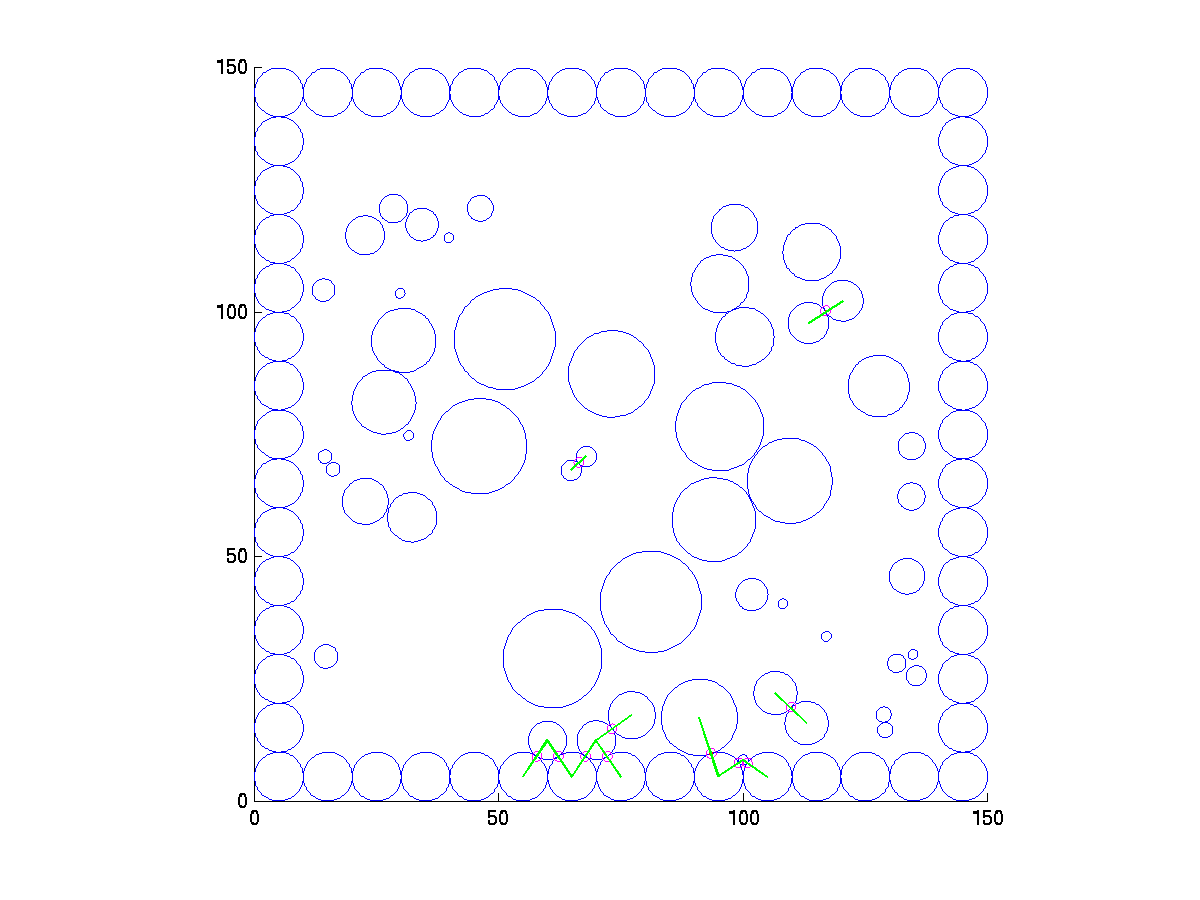
\includegraphics[width=\textwidth]{images/s0110.png}
\end{figure}
This graph suggests either superlinear convergence. The curve bends
slightly downwards.


\begin{figure}[H]
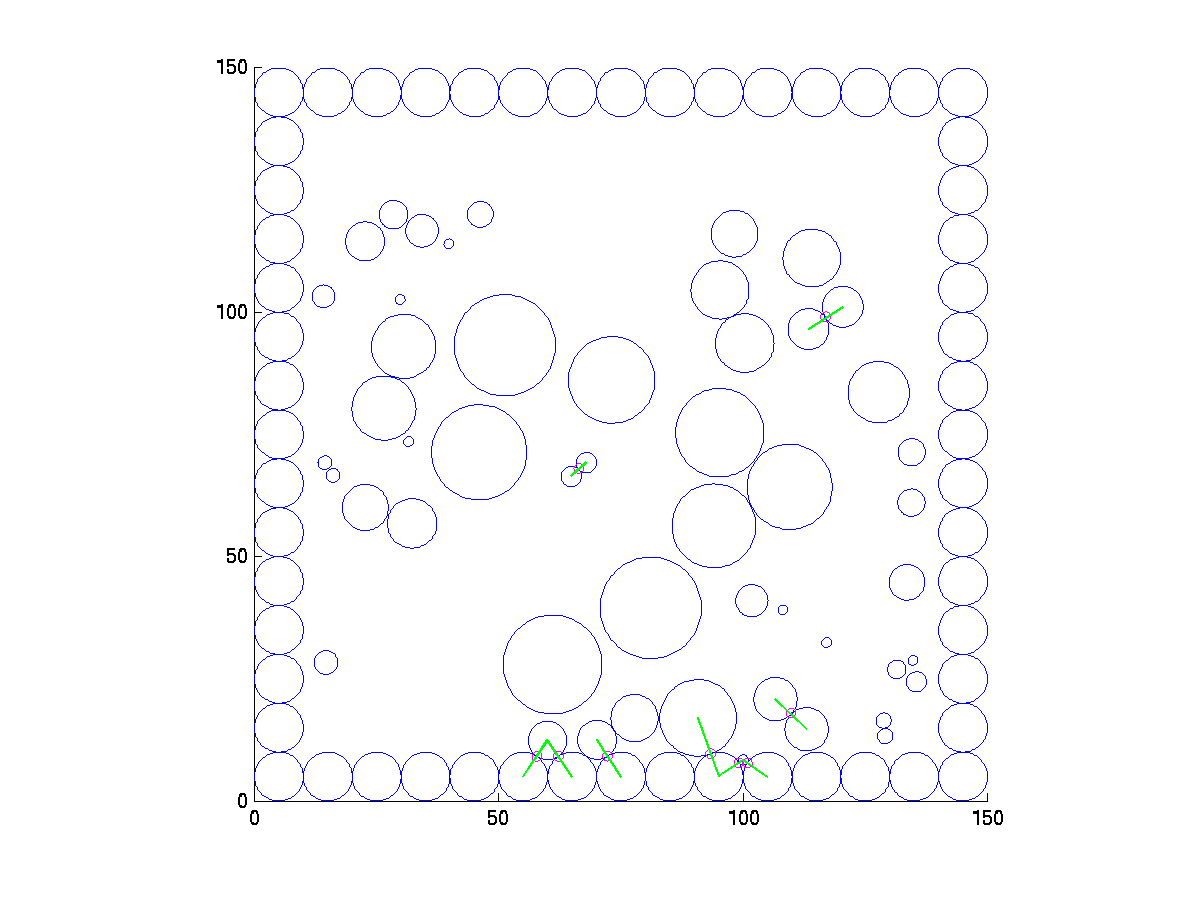
\includegraphics[width=\textwidth]{images/s0115.png}
\end{figure}
This curve from time step 115 also bends downwards. Once again
suggesting superlinear convergence.


\begin{figure}[H]
\includegraphics[width=\textwidth]{images/s1228.png}
\end{figure}
This graph resembles what I see in most of my 250 generated graphs. A
very sharp curve reaching a low error and plenty of iterations. My
terminating condition is an error lower than $0.00001$ or 20000
iterations used. These numbers could probably be lowered, however as I
see it, the bottleneck of the simulation is MatLab's drawing
functions.


This graph shows the number of iterations used throughout each 1000
time steps:
\begin{figure}[H]
\includegraphics[width=\textwidth]{images/total.png}
\end{figure}
It is clear from this graph, that the first 100 iterations or so are
quite simple. Then the problems get more complicated and the number of
iterations go up and variate more. The problems does not seem to get
easier by iteration 1000.


\section{Verification}
In this section, I present my verification of the implementation.


\subsection{Movie of Falling Balls}
I have submitted the movie ``balls.mpg'' together with this paper. It
shows a number of simulation images joined together in a movie. This
movie suggests a correct implementation, since the balls seems to fall
in a ``natural'' way (as natural as I would expect from this
simulation).



% \section{Framework Flow}
% \section{QP Solver}


\section{Conclusion}
I have implemented derived and implemented the Splitting method as
well as investigating its convergence rate. I have shown the relation
between Linear Complementarity Problems and Quadratic Problems. I have
empirically verified the correctness of the implementation by
producing a movie of a simulation (necessary condition for
correctness: Simulations seem OK).


\appendix
\section{Source Code}

\subsection{Run}
\verbatiminput{../code/ball_simulator/run.m}

\subsection{Integrate}
\verbatiminput{../code/ball_simulator/integrate.m}

\subsection{Setup Config}
\verbatiminput{../code/ball_simulator/setup_config.m}

\subsection{Solve LCP}
\verbatiminput{../code/ball_simulator/solve_lcp.m}

\end{document}

%%% Local Variables:
%%% mode: latex
%%% TeX-master: t
%%% End:
